In Cox proportional hazards regression, the outcome considered is time to event. This time should normally be time at risk of an observable event. As an illustration, in Figure \ref{CoxExampleFull}, two subjects are followed until both experience an event (e.g. infection).

\begin{figure}[htp]
	\centering
	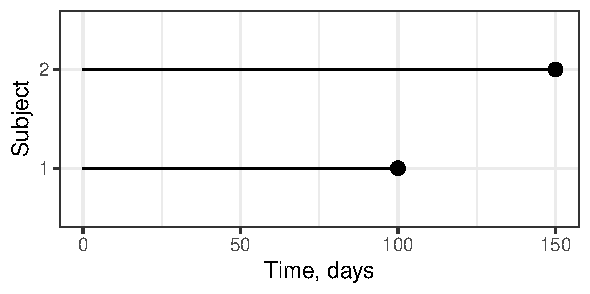
\includegraphics[width=0.6\textwidth]{../curve-cox/timeplot_1_light.pdf}
	\caption{
	An example of time to event data. Two subjects are followed from time 0. Subject 1 experiences the even at time 100. Subject 2 experiences the event at time 150.
	}
	\label{CoxExampleFull}
\end{figure}

Since subject 2 experienced the event later (i.e. ``survived'' for longer), the covariate pattern (e.g. antibody titre) of subject 2 would be considered by the model to be more ``protective'' than that of subject 1.

If subjects are not at risk of the event for all of their follow-up time (e.g. not exposed to the virus), then the total follow-up time may be misleading as illustrated in Figure \ref{CoxExamplePartial}. Taking the actual time at risk into account would lead to the opposite conclusion in this example --- it is subject 1 who is more ``protected'' since they were at risk for longer.

\begin{figure}[htp]
	\centering
	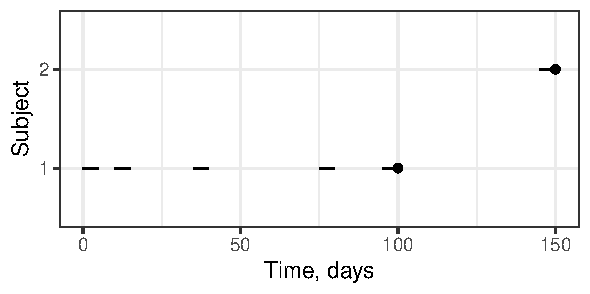
\includegraphics[width=0.6\textwidth]{../curve-cox/timeplot_2_light.pdf}
	\caption{
	An example of time to event data. Two subjects are followed from time 0. Subject 1 experiences the even at time 100. Subject 2 experiences the event at time 150. Subject 1 was at risk of the event for a total of 5 days. Subject 2 was at risk of the event for a total of 25 days.
	}
	\label{CoxExamplePartial}
\end{figure}

\pagebreak

In infection data, true time at risk is unobservable because the risk of infection among susceptible individuals depends on exposure to the pathogen, which cannot be controlled. If follow-up time is completely unrepresentative of true time at risk, the Cox model will not produce reliable results. However, if the total time of follow-up is assumed to be, on average, proportional to the total time at risk (e.g. subjects who are followed up for longer can be expected to have been exposed for longer) then the situation illustrated in Figure  \ref{CoxExamplePartial} will be ``averaged out'' and the model may still produce reliable results.

To investigate this, we generated a simulated dataset, based on the following model:

\begin{align*}
\begin{gathered}
T \sim \text{Exponential}(\text{rate} = \lambda) \\
h(t) = \lambda \\
\text{log}\lambda = -3 - 1.5 X_{\text{logtitre}}
\end{gathered}
\end{align*}

Where $T$ is the survival time, $h$ is the hazard and $X_{\text{logtitre}}$ is the true logtitre measurement simulated from $N(2, 2^2)$.

Each individual was assigned a proportion of time they were exposed to the virus. This proportion was generated from $\text{Beta}(10, 10\frac{1-m}{m})$ where $m$ is the expected proportion for the population. When $m$ was 1, the proportion assigned was always 1 to represent the ideal context of all follow-up time being time at risk. The maximum time of follow-up was set to 200 (days). If an individual's true survival time (a random number generated by $\text{Exponential}(\text{rate} = \text{exp}(-3 - 1.5 X_{\text{logtitre}}) )$ was at most 200 times their ``time at risk proportion'', then they were ``infected''. Otherwise, they were ``not infected''. 

Recorded time for each individual was 200 for everyone not infected (i.e. they were followed for the entire follow-up period and did not experience the event) and the true survival time divided by ``time at risk proportion'' for everyone infected (i.e. they were followed for that amount of time before experiencing the event).

Each simulation included 10,000 observations and was run 10,000 times at different values of the expected proportion of time at risk. The Cox proportional hazards model was fit to each simulated dataset. From 10,000 simulations at each value of the expected proportion at risk, the mean of the estimated coefficient (a measure of its expected value at that proportion) and its standard deviation (a measure of its expected standard error at that proportion and sample size) were saved. The results are summarised in Figure \ref{CoxSimResults}.

In the ideal case (proportion of time at risk set to 1) the estimate is unbiased and has the smallest error. As the proportion of time at risk decreases, bias is introduced while the error remains almost constant. When the proportion is small (less than 20\%), bias appears to decrease while error increases.

The maximum bias was less than 4\% away from the true value. The standard error increases notably only when the expected proportion at risk is very small (less than 10\%). This shows that under the assumption that the time of follow-up is proportional to time at risk, the Cox model can be expected to produce reliable results.

\begin{figure}[htp]
	\centering
	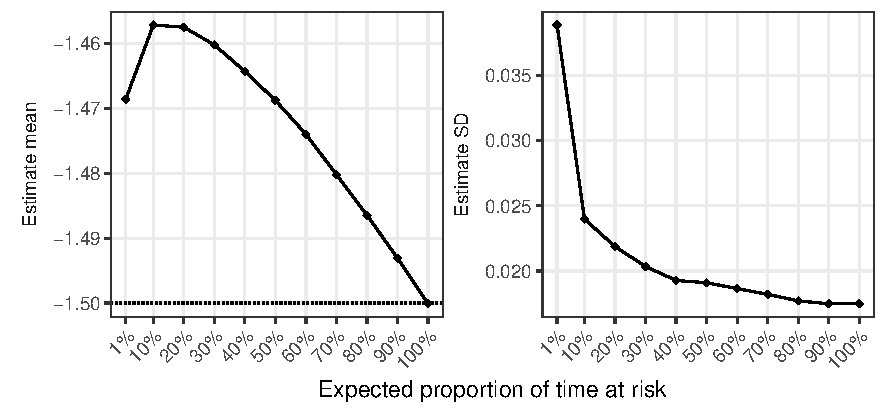
\includegraphics[width=1\textwidth]{../cox-tarprop-plot/risk.pdf}
	\caption{
	The results of time to event simulations. For each proportion of time at risk the mean of the estimated coefficient (left panel) is shown as well its standard deviation (right panel) obtained from 10,000 simulations. Points represent the values of expected proportion for which the simulations were performed. The dotted horizontal line is the true value of the estimated parameter.
	}
	\label{CoxSimResults}
\end{figure}

The assumption of time at risk being proportional to time of follow-up is likely to hold when everyone in the sample is followed through a period of similar disease activity. There may still be subjects who are not exposed (or over-exposed) but as long as the level of exposure does not correlate with the covariates of interest (e.g. antibody titres), then with a large enough sample size the average exposure for any covariate pattern (e.g. antibody titre level) should be proportional in the same way to the time of follow-up. If the disease is seasonal, the start of follow-up can be set to the start of the season. For those who do not get infected, end of follow-up can then be the end of the season. For those who do get infected, end of follow-up can be the infection time assuming that infection grants immunity for the rest of the season. An illustration is in Figure \ref{CoxIdeal}.

\begin{figure}[htp]
	\centering
	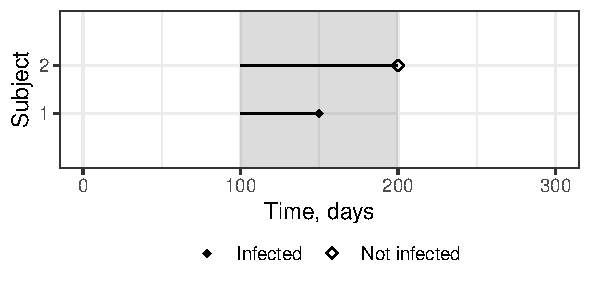
\includegraphics[width=0.59\textwidth]{../curve-cox/timeplot_3_light.pdf}
	\caption{
	An illustration of a pattern of follow-up where the assumption of true time at risk being proportional to time of follow-up is likely to hold. The shaded region marks the period of time when the disease is active. Both subject's follow-up starts at the beginning of the disease season (activity). Subject 1 gets infected at 150 days, their follow-up would end there assuming infection grants immunity (their total recorded time of follow-up would be 50 days). Subject 2 does not get infected through the season, their time of follow-up ends at the end of the season (their total recorded time of follow-up would be 100 days).
	}
	\label{CoxIdeal}
\end{figure}

The assumption will likely not hold if, with a seasonal disease, there are people in the sample whose follow-up starts before the season. An illustration is in Figure \ref{CoxNotIdeal}. For those with earlier follow-up start, their follow-up time will be large regardless of their titres (since they spend a proportion of that time not being at risk). This should make it seem like the titres have a smaller effect than they actually do thus biasing the estimate of titre effect towards the null.

\begin{figure}[htp]
	\centering
	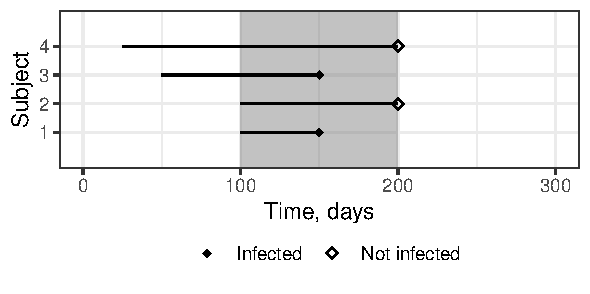
\includegraphics[width=0.59\textwidth]{../curve-cox/timeplot_4_light.pdf}
	\caption{
	An illustration of a pattern of follow-up where the assumption of true time at risk being proportional to time of follow-up is likely to not hold. The shaded region marks the period of time when the disease is active. Subject 1 gets infected at 150 days, at which point their follow-up would end if it can be assumed that infection grants immunity (their total recorded time of follow-up would be 50 days). Subject 2 does not get infected within the season, their follow-up ends at the end of the season (their total recorded time of follow-up would be 100 days). For subjects 3 (recorded follow up of 100 days) and 4 (recorded follow-up of 175 days) follow-up commenced prior to season onset.
	}
	\label{CoxNotIdeal}
\end{figure}

%\pagebreak

To demonstrate this problem, we performed some additional simulations using the same procedure as described above except subjects were randomly chosen to have had their follow-up started earlier. For those chosen, a uniform random number between 0 and 200 (days) was added to their recorded follow-up time. The proportion of time at risk was set to 1. The bias resulting from varying the proportion of the sample with earlier follow-up is shown in Figure \ref{CoxSimLong}. The estimate is unbiased when follow-up starts at the start of the season. Bias towards the null increases rapidly even when only a small (10\%) proportion of the sample has started follow-up prior to the season. For this reason, it would be advisable to record follow-up time in such a way so that true unobservable time at risk can be reasonably expected to be proportional to the recorded time of follow-up (i.e. the longer a subject is followed, the longer they are likely to have been at risk).

\begin{figure}[htp]
	\centering
	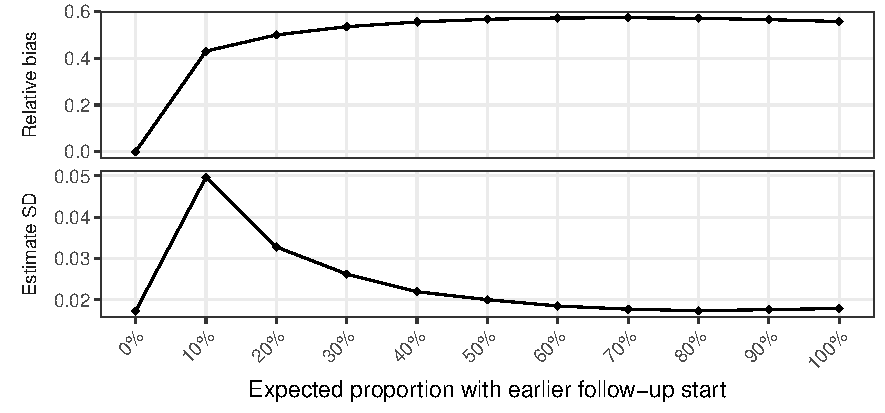
\includegraphics[width=1\textwidth]{../cox-tarprop-plot/long.pdf}
	\caption{
	The results of time to event simulations. For each proportion of the sample with earlier follow-up start, the mean of the estimated coefficient (left panel) is shown as well as the standard deviation of that coefficient (right panel) from 10,000 simulations. Points represent the values of expected proportion for which the simulations were performed. The dotted horizontal line is the true value of the estimated parameter.
	}
	\label{CoxSimLong}
\end{figure}
